% =========================================================================
% ICRA 2027 submission, 6-page cut. Paper 1 of two.
% =========================================================================
% This file is the SUBMISSION. main.tex is the long source (~10 pages) and
% stays as the archive: the merge tables, the drift sweep and the
% conditioning ablations cut from here are the raw material for paper 2
% (merge, joint with Shay, on VSA-OGM's Intel benchmark). Do not delete
% material from main.tex to "sync" the two files.
%
% Thesis of this cut: fixed size is not the contribution; PREDICTED
% degradation is. The capacity law is the headline, not the third of four.
%
% Class note: written against IEEEtran conference mode. ICRA's PaperPlaza
% template is ieeeconf.cls; swap is one line:
%   \documentclass[letterpaper, 10pt, conference]{ieeeconf}
%
% Every number traces to the tracker
% (wiki/analysis/2026-07-29-vsa-query-layer-paper-plan.md) or a named
% artifact. Provenance lives ONLY in "% provenance:" comments.
% =========================================================================
\documentclass[conference]{IEEEtran}
\IEEEoverridecommandlockouts

\usepackage{amsmath,amssymb}
\usepackage{booktabs}
\usepackage{graphicx}
\usepackage{xcolor}
\usepackage{url}
\usepackage{cite}
\usepackage[hidelinks]{hyperref}
\usepackage{cuted}
\usepackage{capt-of}

\newcommand{\todo}[1]{\textcolor{red}{\textbf{[TODO: #1]}}}
\newcommand{\bnd}{\odot}
\newcommand{\conj}[1]{\overline{#1}}

\begin{document}

\title{Algebraic Spatio-Temporal Memory: a Fixed-Size Vector-Symbolic Map
with a Predictive Capacity Law}

% Author order per Paul, 2026-08-10.
\author{
\IEEEauthorblockN{
Sven Krausse\IEEEauthorrefmark{1},
Shay Snyder\IEEEauthorrefmark{2},
Naitri Rajyaguru\IEEEauthorrefmark{3},
Lorin Achey\IEEEauthorrefmark{4},
Paul Kirkland\IEEEauthorrefmark{5}}
\IEEEauthorblockA{
\IEEEauthorrefmark{1}Peter Gr{\"u}nberg Institute, Forschungszentrum
J{\"u}lich, and RWTH Aachen University, Germany\\
\IEEEauthorrefmark{2}Parsa Research Laboratory, George Mason University,
Fairfax, VA, USA\\
\IEEEauthorrefmark{3}Perception and Robotics Group, University of
Maryland, College Park, MD, USA\\
\IEEEauthorrefmark{4}Collaborative AI and Robotics Lab, University of
Colorado Boulder, CO, USA\\
\IEEEauthorrefmark{5}International Centre for Neuromorphic Systems
(ICNS), The MARCS Institute, Western Sydney University, Australia\\
\todo{contact email for the corresponding author}}}

\maketitle

% =========================================================================
\begin{abstract}
Semantic maps on robots are usually structures that grow: a node per
object, a row per landmark, a descriptor per keyframe. We characterise
the opposite design point, a spatial-semantic map whose entire state is
one fixed-size vector, and argue that fixed size is not by itself the
contribution. Bounded-memory representations already exist; what they
lack is a model of their own degradation, so they fail silently as
content approaches capacity. Observations are bound to positions by
elementwise complex multiplication over Fourier Holographic Reduced
Representation phasors and superposed into a single 32\,KB trace
($D=8192$ unit-modulus phasors stored as phase angles alone, one float32
per dimension; 64\,KB under the complex64 convention); queries about
objects, places and times are answered by the algebra's inverse
operation in milliseconds on a laptop CPU, with no structure to
traverse. Our central contribution is an empirical capacity law for
superposition interference that separates a mean term, a quadrature
content/projection term and a temporal-persistence factor. It predicts a
held-out condition to 1.4\%, it diagnosed a deployed class-imbalance
failure and predicted the direction of the bounded-insertion fix that
repaired it, and it is what allows a single trace to stay single where
comparable systems tile for want of a capacity model. We characterise
the cost of the budget on real perception: cross-traverse relocalisation
on 7-Scenes \texttt{chess} reaches 0.36\,m median 3D error from the
trace against 0.29\,m for exact nearest neighbour over the same
descriptors at 32.8\,MB, and object grounding across all eight Replica
scenes leaves zero memory-attributable misses. Against ConceptGraphs
under its own Replica evaluation --- the baseline first reproduced to
99\% of its published score --- the 32\,KB trace reaches 0.80$\times$
the unbounded map's accuracy on clean input and \emph{overtakes it
outright} in all nine degraded-input conditions tested: predicted
degradation is what the fixed budget buys. The memory does not exceed
the ceiling its perception sets.
\end{abstract}

% Page-1 teaser. A figure* cannot appear on the page it is declared on,
% so this uses cuted's strip (not a float) plus capt-of.
% Regenerate with:  python tools/make_hero_figure.py
\begin{strip}
\centering
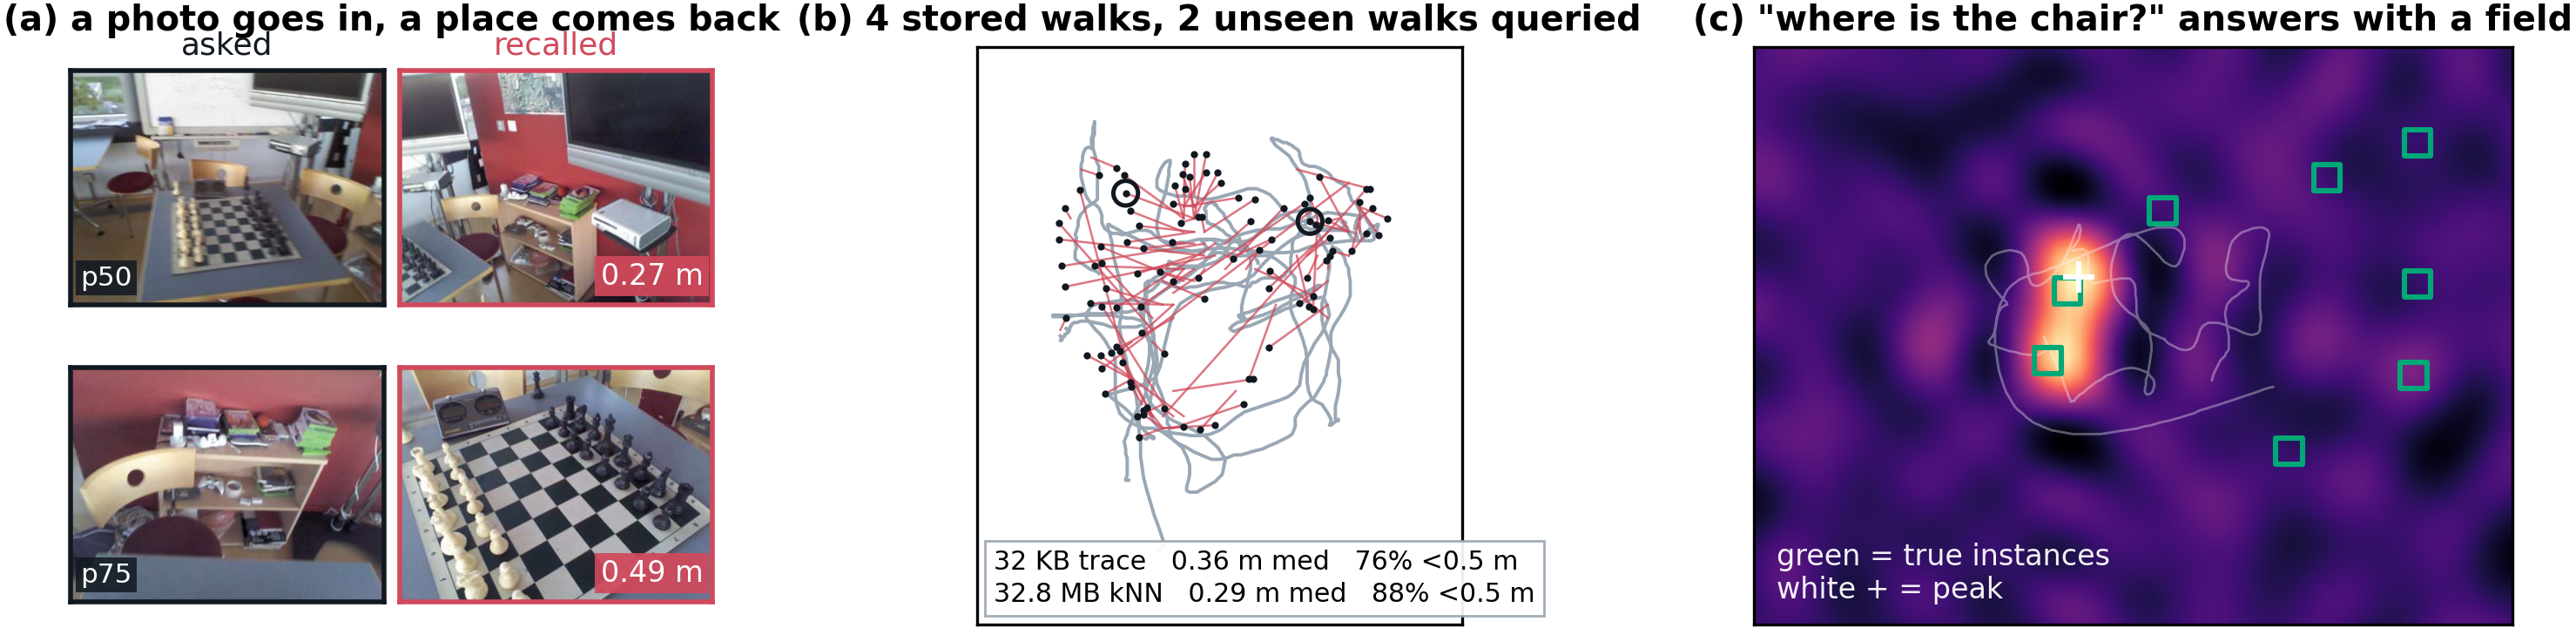
\includegraphics[width=\textwidth]{figures/hero.png}
\captionof{figure}{The whole system, drawn from its own state. Every
vector is shown as its phase angles and every one was computed by our
implementation from the real Replica \texttt{room0} stream.
\textbf{(a)} An observation is one multiply-add: a content atom bound to
a fractional-power position code (Eq.~\eqref{eq:fpe}), added into a
running sum. \textbf{(b)} The whole map is that sum --- 8{,}192 phases at
4 bytes each, 32\,KB (Sec.~\ref{sec:traces} on the byte convention), a
size fixed before the robot moves and unchanged by how much it then sees.
\textbf{(c)} A question is one unbind: dividing by the \texttt{chair}
atom leaves a spatial belief \emph{field} over the floor rather than a
lookup result, and the field is the map's full answer where argmax is one
readout of it. \textbf{(d)} Two maps combine by addition, equalling the
jointly built map with no data association whatsoever.
\todo{regenerate panel (c) from the real-GT grounding branch --- the
current render is from the provisional pseudo-session split, so its
markers are second-half cluster centroids and its memory is a half-walk.
Restore the ``every ground-truth instance'' wording only after that.}}
\label{fig:hero}
\end{strip}

% =========================================================================
\section{Introduction}
\label{sec:intro}

A mobile robot's semantic map is usually a data structure that grows: a
3D scene graph adds a node per object and edges per relation
\cite{hughes2022hydra,gu2024conceptgraphs}, a landmark map adds a row per
landmark, a view database adds a descriptor per keyframe. Growth is not
the problem by itself; the machinery it obligates is. Updating a growing
structure means data association; merging two of them means
correspondence solving, outlier rejection and joint optimisation
\cite{tian2022kimeramulti,chang2023hydramulti}; and every downstream
query needs code that \emph{traverses} the structure, walking it element
by element until it finds what the query asked for.

Bounding that growth is now a named problem with its own survey. Across
roughly 52 systems from 1989 to 2025, Pangaliman et al.\
\cite{pangaliman2026memorysurvey} taxonomise spatial memory as dense,
sparse, neural or hierarchical-semantic, and quantify the gap between
stored map and runtime cost as the ratio of peak runtime memory to saved
map size --- a ratio reaching 215 for a 47\,MB neural map. Their critique
of the systems that \emph{do} bound size is the objection this paper
exists to answer: hash-based maps cap the table, but quality ``degrades
silently when scene complexity approaches table capacity, providing
bounded memory rather than constant-quality scaling.''

That sentence sets our thesis. Fixed size is not the contribution.
\emph{Predicted} degradation is. This paper characterises a map that does
not grow --- a robot that has driven for an hour and a robot that has
driven for a week hand over the same object, 8{,}192 phase angles at four
bytes each --- and, more importantly, supplies the law that says when
that object saturates, by how much, and what to do about it.

We build the map from a vector symbolic algebra (VSA; the older
literature reads the acronym as ``architecture''), used as an
\emph{algebraic composition layer}. Class, appearance, position, heading
and time are each encoded as high-dimensional unitary phasor vectors,
composed by one binding operator, and superposed into a map state whose
size is fixed \emph{before} the robot ever moves: 32\,KB in every
experiment here. Insertion is one multiply-add, $O(D)$. A family of
spatial-semantic queries (``where was a chair?'', ``what is at
$(x,y)$?'', ``when was this place occupied?'') is answered by a single
unbind followed by a kernel readout; nothing walks a structure, because
there is no structure to walk. Merging two maps is elementwise addition:
commutative, associative and exact, because a representation that makes
no association decisions has none for a merge step to get wrong.

Because everything shares one superposition, the memory's interference
has a closed form. Section~\ref{sec:law} gives that law, $\chi(N)$,
separately evidencing its three terms, validating it on a held-out
condition to 1.4\%, and showing that it called a class-imbalance failure
on real scenes in advance together with the fix that repaired it. This
is the capability that distinguishes the design point rather than the
byte count: a comparable VSA mapping system \cite{snyder2026vsaogm}
partitions its environment into per-region memory vectors and lists
saturation as an open limitation precisely because no such law was
available to it.

We are equally explicit about what is not claimed. The memory does not
out-localise a nearest-neighbour search over its own input descriptors;
superposition is lossy, and lossy representations lose. A detector-fed
object memory cannot label the walls and floors that dominate dense
semantic-segmentation benchmarks, so we pre-register that expectation
under the target benchmark's own scorer rather than choosing a protocol
that hides it (Sec.~\ref{sec:grounding}). Exact merging assumes a shared
coordinate frame, which is precisely what the classical merge machinery
exists to recover. Instance identity is a stated limitation. The claims
are about what a fixed-size algebraic map state buys \emph{at the ceiling
its perception sets}.

Contributions:
\begin{enumerate}
\item \textbf{Capacity law} (Sec.~\ref{sec:law}): an empirical law for
  superposition interference, $\chi(N)$, separating a mean term, a
  quadrature content/projection term, and a temporal-persistence factor;
  it predicts a held-out condition to 1.4\% and correctly anticipated a
  deployed failure and its fix. It is what lets one fixed-size trace stay
  single.
\item \textbf{System} (Sec.~\ref{sec:method}): a fixed-dimensional
  associative map over real perception --- FHRR traces with fractional
  power encoding, bounded per-class insertion, and a content-conditioning
  discipline (centre or z-score, or bind a diverse key; the two are
  measured substitutes) --- together with the byte convention its
  headline number depends on.
\item \textbf{Benchmark characterisation} (Sec.~\ref{sec:results}):
  cross-traverse relocalisation on 7-Scenes \texttt{chess} against
  storage-matched and storage-unmatched baselines; object grounding on
  all eight Replica scenes with a full miss taxonomy; and a head-to-head
  against ConceptGraphs under its own evaluation --- baseline reproduced
  to 99\% of published first --- including a matched degradation study
  in which the bounded memory overtakes the unbounded map in every
  condition tested.
\end{enumerate}

% =========================================================================
\section{Related Work}
\label{sec:related}

\textbf{Vector symbolic algebras.} Holographic reduced representations
\cite{plate1995holographic} and hyperdimensional computing
\cite{kanerva2009hyperdimensional,kleyko2022survey} compose symbols in a
fixed-dimensional space via binding and superposition, with capacity
analyses assuming i.i.d.\ quasi-orthogonal vectors \cite{frady2018theory}.
Continuous space enters through fractional power encoding
\cite{komer2019neural,voelker2021simulating}, deployed in spiking form by
SSP-SLAM \cite{dumont2023sspslam} and as a grid-cell-inspired structured
algebra by Krausse et al.\ \cite{krausse2025gcvsa}. HyperSpace
\cite{snyder2026hyperspace} formalises the bind-then-bundle write and its
inverting query as the storage and query modules of a general spatial-VSA
framework; we take that primitive as given and ask what a \emph{fixed}
budget of it buys on real perception, where the randomness assumptions
fail (Sec.~\ref{sec:law}).

\textbf{Bundling as a merge operator.} HDC aggregation of image
descriptors exists \emph{within} an agent for place recognition
\cite{neubert2021hyperdimensional} and across clients in federated
learning \cite{fedhd2022}. Closest to us, VSA-OGM \cite{snyder2026vsaogm}
merges maps \emph{between} robots by bundling, on a synthetic LiDAR scene
and on Intel Campus quadrants. Two differences matter here. It bundles
occupancy --- binary occupied/empty classes over a tiled grid of memory
vectors --- where we bundle a spatial-semantic memory binding class,
appearance, position, heading and time. And it \emph{tiles} rather than
bundling into one vector, listing memory-vector saturation as an open
limitation: as point counts grow, dimensionality or tile count must grow
with them. That is a published VSA mapping system backing away from the
single fixed-size vector for want of a capacity model, which is the gap
Sec.~\ref{sec:law} fills.

\textbf{Scene graphs and open-vocabulary maps.} Hydra
\cite{hughes2022hydra}, ConceptGraphs \cite{gu2024conceptgraphs},
ConceptFusion \cite{jatavallabhula2023conceptfusion}, HOV-SG
\cite{werby2024hovsg} and successors \cite{keysg2025} build exact,
mutable, relational structures with open-vocabulary semantics. These
systems and ours occupy different corners of a real trade-off:
exact/mutable/growing state versus bounded/associative/approximate state.
Two 2026 results sharpen it in the graphs' favour on bytes, and we state
that rather than let a reviewer state it for us. Clio
\cite{maggio2024clio} compresses a graph by an agglomerative information
bottleneck over natural-language tasks; LOST-3DSG
\cite{ferraina2026lost3dsg} replaces dense CLIP attributes with word2vec
and sentence embeddings, representing a 21-object scene in 3{,}297 bytes
--- an order of magnitude below our trace, with instance identity intact,
which is exactly what Sec.~\ref{sec:limitations} concedes we lack. Small
is therefore not our differentiator and we do not argue it. What no
explicit representation offers is a footprint fixed \emph{before}
deployment, an update cost independent of map age, a merge cost
independent of map content, and a law for its own degradation. We adopt
ConceptGraphs' own evaluation for the semantic comparison
(Sec.~\ref{sec:grounding}) rather than inventing a metric. Relational
spatial memories with referring-expression interfaces \cite{farm2026}
mark the expressiveness frontier this representation does not reach.

\textbf{Relocalisation.} Retrieval-based relocalisation stores a
descriptor database and returns the pose of the best match
\cite{sattler2019understanding}; compression via product quantisation
\cite{jegou2011product} trades accuracy for bytes but is floored by its
codebook. We use 7-Scenes \cite{shotton2013scene} with EigenPlaces
descriptors \cite{berton2023eigenplaces} and treat exact nearest
neighbour over the same descriptors as the ceiling the memory should
track.

% =========================================================================
\section{Method: the Algebraic Map}
\label{sec:method}

\subsection{Encoding}
\label{sec:encoding}

All atoms are unitary phasor vectors $z \in \mathbb{C}^{D}$ with
$z_j = e^{i\theta_j}$, $\theta_j \sim \mathcal{U}[-\pi,\pi)$, at
$D=8192$ throughout. Binding is the elementwise complex product
$a \bnd b$; unbinding is binding with the conjugate; superposition is
vector addition. A discrete symbol is one random atom; continuous
quantities use \emph{fractional power encoding} \cite{komer2019neural}:
a base atom $X$ is exponentiated elementwise,
\begin{equation}
S(x) \;=\; X^{x} \;:=\; e^{\,i x \boldsymbol{\theta}_X}, \qquad
S(x,y) = X^{x} \bnd Y^{y},
\label{eq:fpe}
\end{equation}
which makes position encoding a group homomorphism,
$S(a) \bnd S(b) = S(a+b)$ --- exact to machine precision in our
implementation ($1.5\times10^{-16}$ max deviation over a $4\times4$
displacement sweep), so translating a whole belief field costs one bind.
The similarity $\langle S(x), S(x')\rangle$ is a fixed radial kernel with
length-scale $\ell$ (0.5--0.75\,m indoors). Heading uses a circular base
atom with integer frequencies $\pm\{1,2,3\}$ and no DC component, so
marginalising heading out of a query costs one bundled probe.

\subsection{Map state, and what a byte is}
\label{sec:traces}

An observation of content $c$ (a class atom, an appearance phasor, or
their binding) at position $(x,y)$ is inserted by one multiply-add:
\begin{equation}
M \;\leftarrow\; M + c \bnd S(x,y).
\label{eq:insert}
\end{equation}
A query for $c$ produces a spatial belief field by unbinding and kernel
readout,
\begin{equation}
f(x) \;=\; \operatorname{Re}\,\langle\, M \bnd \conj{c},\; S(x)\,\rangle,
\label{eq:field}
\end{equation}
evaluated over a display grid; the answer is the field's argmax, and we
recommend reporting the top-$k$ modes. The field \emph{is} the map;
argmax is one readout of a full spatial belief. Because a trace answers
best the query shape it was built for, the memory keeps one trace per
query family --- $\sum c \bnd S(x)$, $\sum c \bnd T(t)$,
$\sum S(x) \bnd T(t)$, and a full event trace $\sum c \bnd S(x) \bnd T(t)$
--- in effect the algebra's secondary indexes, each carrying its own
capacity budget under Sec.~\ref{sec:law}.

At $D=8192$, one trace is 8{,}192 phase angles at 4 bytes: 32\,KB.
\emph{This convention is load-bearing.} Because the phasors are
unit-modulus, the map state is the phase angles alone, one float32 per
dimension. The standard FHRR accounting stores a complex64 pair per
dimension and would give $8D = 64$\,KB \cite{snyder2026hyperspace}; the
magnitudes it stores are the constant we never need. Byte counts here use
the phase-only convention, and doubling them recovers the complex64
reading. The trace is the \emph{map state}: the decode grid used to
display a field is working memory derived from the shared basis, and
dense decoding dominates query latency ($\sim$91\% in profiling) but is
not needed by consumers that stay in the algebra. HyperSpace
\cite{snyder2026hyperspace} measures the same effect independently and
from a different pipeline --- similarity-driven cleanup and regression
dominate end-to-end runtime, to the point where HRR and FHRR come out
comparable despite FHRR's cheaper operators. The saving is available only
to consumers that never decode. Query latency is milliseconds on a laptop
CPU (2.7--15\,ms across our configurations at $D=4096$--8192).

\subsection{Bounded per-class insertion}
\label{sec:bounded}

Class frequencies in real streams are heavy-tailed, and the capacity law
predicts the consequence: a class stored 1{,}150 times buries one stored
5 times under crosstalk mass (Sec.~\ref{sec:law}). Insertion is therefore
capped per content symbol (reservoir-style, $\le 60$ insertions per
class), which is online, requires no second pass, and preserves merge
exactness by construction. On Replica \texttt{room0} this raised
provisional consistency-R@1 from 44\% to 62\% exactly as the law's
direction predicted; the final truth-scored protocol grounds 5 of 6
GT-comparable classes (83\%).
% provenance: tracker (ba->bb); outputs/replica_room0/object_grounding.json
% (metric 'truth'); the 44->62 pair is the provisional consistency metric

\subsection{Content conditioning, and a substitution law}
\label{sec:conditioning}

Learned perception features violate the i.i.d.-random assumption of VSA
capacity theory in one dominant way: a shared mean direction that
accumulates \emph{coherently} across stored items. Two measured rescues
exist, and they substitute for each other. \emph{(1) Condition the
content stream}: centre, or z-score per dimension, using statistics fit
on memory-building data only. Full whitening is not a stronger version of
this fix --- it flattens the spectrum, which is where retrieval lives,
and scores below a constant predictor in most held-out cells ($-47.6\%$
signal, classroom EigenPlaces, 5 seeds); its effect is scene- and
encoder-dependent, so we state it as scoped. \emph{(2) Bind a diverse
key}: a third bound factor whose value varies across insertions (e.g.\
heading) scatters the shared mean's phases, destroying the coherent
pile-up by the key rather than by preprocessing; on streams where content
is nearly parallel this rescues a degenerate memory outright ($-38.7\%$
signal, decode collapsed to one cell, $\to +63.3\%$).
% provenance: tracker (am)
Use exactly one. Binding an \emph{uninformative} extra key when content
is already conditioned adds pure crosstalk (0.35\,m $\to$ 1.00\,m), and
whether a key is informative is trajectory-dependent
(Sec.~\ref{sec:chess}).

\subsection{Merge}
\label{sec:merge-method}

Two traces built under a shared atom vocabulary and a shared coordinate
convention merge by elementwise addition, $M_{A\cup B} = M_A + M_B$:
commutative, associative, content-independent in cost, and exact up to
floating-point reordering, with no association decisions because there
are no discrete elements to associate. Bundling as a between-agent merge
operator is established for occupancy \cite{snyder2026vsaogm}; what
addition does \emph{not} provide is the shared frame itself, which is
precisely the problem the classical machinery solves. Misaligned traces
sum to a superposition of inconsistent maps with no error signal. A
measured comparison against association-based merging is the subject of a
companion paper; Sec.~\ref{sec:merge-results} reports only the check that
bears on this one.

% =========================================================================
\section{A Predictive Capacity Law}
\label{sec:law}

\subsection{Metric}
Store $N$ items, probe with a stored key, and measure the response at
non-target locations in units of one item's on-target signal:
\begin{equation}
\chi(N) \;=\; N \cdot \operatorname{mean}_i \left| \text{off-target}_i \right|,
\label{eq:chi}
\end{equation}
the interference amplitude per unit item signal ($\chi$ values are
comparable only at matched $N$). Retrieval flips when interference mass
competes with the on-target peak, so $\chi$'s growth in $N$ \emph{is} the
capacity story. This is the quantity whose absence forces tiling
elsewhere \cite{snyder2026vsaogm}; a law for $\chi$ is what lets a single
fixed-size trace stay single.

\subsection{The law}
Across controlled synthetic sweeps ($N$ to $10^6$; Fig.~\ref{fig:law})
and real encoder streams, interference follows
\begin{equation}
\chi(N) \;=\; a_\mu N \;+\; \sqrt{N}\,
\sqrt{\tfrac{\alpha}{\mathrm{PR}_{\mathrm{eff}}} + \tfrac{\gamma}{D}}\;
h(N,\tau),
\label{eq:law}
\end{equation}
with three separately-evidenced components.
% provenance: tracker (az); wiki/analysis/2026-08-04-t1-chi-law-empirics.md;
% outputs/synthetic/rows.jsonl + outputs/synthetic_hd1024/rows.jsonl

\textbf{Mean term, exactly linear.} A shared mean direction adds in
phase: $\chi/N$ is constant to $3\times10^{5}$ items (0.0083 across the
sweep), and configurations without a mean fit $a_\mu \approx 0$. This
term never bends; it is the component the conditioning rules of
Sec.~\ref{sec:conditioning} exist to kill: centring removes it, a diverse
bound key phase-scatters it.

\textbf{Quadrature fluctuation term.} The $\sqrt{N}$ prefactor has two
sources in quadrature: content-space overlap $\alpha/\mathrm{PR}$
(participation ratio of the content covariance, where treatments act) and
a projection-noise floor $\gamma/D$ that is \emph{content-independent}. A
single-power-law alternative was falsified by a $D$=1024 run; the
quadrature model fits all (config$\times D$) cells and predicts a
held-out cell to \textbf{1.4\%} (predicted 0.0321, observed 0.0316). The
$\gamma/D$ term explains a real-data observation: after whitening, four
backbones spanning raw $\chi$ 79.8--201.8 (YOLOv8n, ResNet-50, DINOv2-S,
untrained ResNet-50; $N$=2{,}429, $D$=8192) land on the same floor
($\chi$ 9.1--11.0). No content treatment goes below the projection floor;
only more dimensions can.

\textbf{Persistence factor.} Temporally correlated streams grow
coherently while $N \lesssim \tau$ (the correlation length in items),
then revert to $\sqrt{N}$ with a \emph{permanent} elevation
$h_\infty = \sqrt{1 + \tau/\tau_0}$ ($\tau_0 \approx 60$ at our settings;
elevation$^2-1 \propto \tau$ verified across a 200$\times$ range of
$\tau$). The mean is the $\tau\to\infty$ limit. Practically, naive $O(N)$
extrapolation from small-$N$ measurements \emph{overstates} crosstalk at
scale for everything except the mean term.

\begin{figure}[t]
\centering
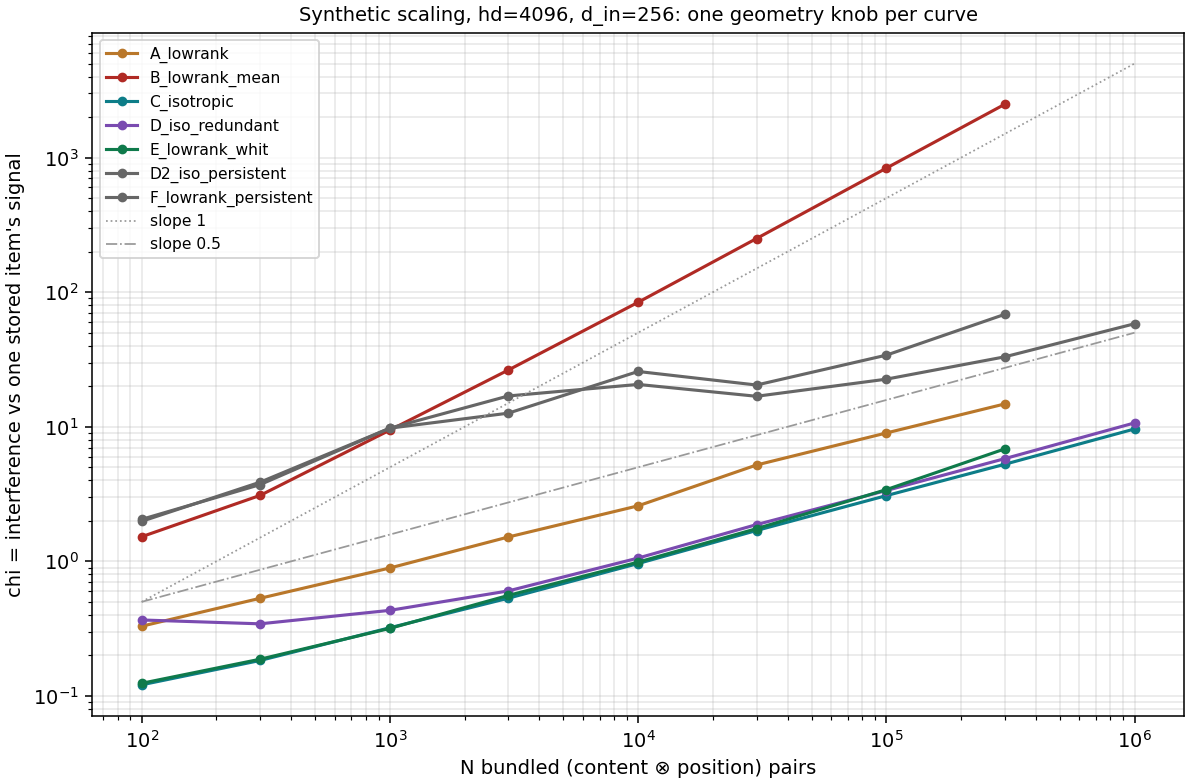
\includegraphics[width=\linewidth]{figures/synthetic_scaling.png}
\caption{Interference growth $\chi(N)$ on controlled synthetic content
streams through the exact deployed pipeline. A shared mean grows
coherently ($O(N)$, never bends); anisotropic-but-independent content
grows at $\sqrt{N}$ with a larger prefactor; temporally persistent
content is transiently coherent then reverts. These are the three terms
of Eq.~\eqref{eq:law}. \todo{regenerate with legend labels matching the
equation terms}}
\label{fig:law}
\end{figure}

\subsection{Deployed predictions}
The law is not descriptive bookkeeping; it does live diagnostic work.
\emph{(i) Class imbalance}: heavy-tailed insertion counts put a large
coherent mass on frequent classes --- the mean term at class granularity
--- predicting that rare classes drown; the law predates the deployment
that exhibited it, and it predicted the fix's direction before the fix
was applied. Measured: couch at 1{,}150
insertions buried book at 5; bounded insertion (Sec.~\ref{sec:bounded})
raised all-class grounding 44\%$\to$62\%. \emph{(ii) The
encoder-independent floor}: the $\gamma/D$ term, measured on four
backbones above. \emph{(iii)} Two falsifiable predictions are on record:
doubling $D$ halves the whitened floor's squared prefactor but barely
moves a content-dominated raw encoder, and halving frame rate halves
$\tau$, lowering the large-$N$ asymptote by a predicted factor.

The practical form of the law is a deployment discipline. Condition the
content stream or bind a diverse key, never both; cap per-class
insertion; and read off, before deployment, the $N$ at which a given $D$
stops answering. That is what a bounded memory needs in order not to
degrade silently \cite{pangaliman2026memorysurvey}.

% =========================================================================
\section{Experiments}
\label{sec:results}

\textbf{Datasets.} (i) 7-Scenes \texttt{chess} \cite{shotton2013scene},
official split: memory from the 4 training walks (4{,}000 frames),
queries from the 2 physically separate test walks (2{,}000 frames).
(ii) Replica \cite{straub2019replica}, all 8 scenes, using the
NICE-SLAM/vMAP rendered sequences \cite{zhu2022niceslam,kong2023vmap};
ground-truth instances come from backprojected per-pixel instance
renders with a frame-alignment gate. (iii) A self-collected Spot
classroom sequence (2{,}429 frames, LIO-SAM poses) for conditioning
ablations.

\textbf{Frontends.} Whole-frame EigenPlaces descriptors
\cite{berton2023eigenplaces} for place queries; YOLOv8n
\cite{jocher2023yolov8} detections deprojected through depth for objects;
DINOv2-S \cite{oquab2023dinov2} and CLIP \cite{radford2021clip} where
noted. The memory never estimates pose: it is handed a pose per frame,
stores content bound to it, and returns stored poses associatively.

\textbf{Protocol discipline.} No random train/test splits on video --- at
15\,fps a held-out frame's neighbours remain stored, the oracle collapses
to 0.01\,m and an untrained encoder ties DINOv2 --- so we use contiguous
blocked splits or physically separate traverses. Every retrieval number
is bracketed by chance, an oracle and a constant predictor, and reported
as a distribution rather than a median alone. Where a comparison targets
a published system we adopt that benchmark's metric, scorer and ground
truth verbatim; protocols of our own design are labelled characterisation
and never presented as comparable numbers. Conditioning statistics are
fit on memory-building data only.

\subsection{Relocalisation at 32\,KB}
\label{sec:chess}

Table~\ref{tab:chess} gives the storage/accuracy trade at a fixed
frontend (EigenPlaces, z-scored on memory statistics). Exact kNN over all
stored descriptors is the ceiling; product quantisation
\cite{jegou2011product} is the standard compression; the trace is
$\sim$1000$\times$ smaller than the ceiling and lands 0.07\,m from it in
median 3D error (0.36 vs.\ 0.29\,m). PQ at $m$=8 is excellent at 2.1\,MB but \emph{cannot exist} at
32\,KB, since its $256\times2048$ codebook alone is $\sim$2\,MB, so the
trace occupies a size regime with no PQ counterpart at this $N$. Our kNN
ceiling (0.29\,m) is the class of published retrieval baselines on this
scene \cite{sattler2019understanding}. Top-3 readout closes most of the
argmax gap
(2D $\le$0.5\,m: 76.4\%$\to$91.5\%), consistent with truth sitting near a
secondary mode of the belief field.

\begin{table}[t]
% provenance: tracker (ax); outputs/cross_recall_7scenes_chess.json
\caption{7-Scenes \texttt{chess}, official cross-traverse split
(memory = 4 train traverses, queries = 2 test traverses; EigenPlaces
z-scored; $D$=8192). Trace bytes are phase-only
(Sec.~\ref{sec:traces}); under the complex64 convention the trace reads
64\,KB and the comparison is unchanged in kind.}
\label{tab:chess}
\centering
\small
\begin{tabular}{@{}lrrrr@{}}
\toprule
System & Bytes & 3D med. & \multicolumn{2}{c}{2D fraction} \\
 & & & $\le$0.5\,m & $\le$1\,m \\
\midrule
kNN exact (ceiling) & 32.8\,MB & 0.29\,m & 88.5\% & 98.1\% \\
PQ $m{=}8$ & 2.1\,MB & 0.29\,m & 89.6\% & 98.5\% \\
kNN, storage-matched fp16 & 32\,KB & \todo{run} & \todo{} & \todo{} \\
\textbf{VSA trace} & \textbf{32\,KB} & \textbf{0.36\,m} & 76.4\% & 93.0\% \\
VSA top-3 (2D) & 32\,KB & -- & 91.5\% & 98.9\% \\
\bottomrule
\end{tabular}
\end{table}

The conditioning mechanism replicates on this public benchmark: the raw
trace reaches only 0.75\,m median 3D versus 0.37/0.36\,m
centred/z-scored. Two scoped nuances, both measured: whitening is
harmless \emph{here} (0.34\,m) though strongly harmful elsewhere, so the
claim is scene- and encoder-dependent and never stated universally; and
binding heading mildly helps the tail on this orbit-style scene (argmax
$\le$1\,m: 93.0\%$\to$97.9\%), so the substitution law's
``uninformative key'' clause is trajectory-dependent.

\subsection{Object grounding on eight Replica scenes}
\label{sec:grounding}

We characterise the object memory with a protocol of our own design and
label it as such: store the YOLO+depth object stream (bounded insertion,
one 32\,KB trace per scene, 2{,}357--10{,}465 observations); query each
ground-truth-comparable class; an answer grounds correctly if the decoded
position lies within $r$ of a true instance of that class, with
Monte-Carlo chance anchors. Pooled over 8 scenes and 42 scoreable GT
classes (37 of 42 ground correctly at $r$=1\,m): 88.1\% at $r$=1\,m
(chance 18.2\%) and 78.6\% at $r$=0.5\,m (chance 5.9\%).
% provenance: tracker (bd); outputs/replica_truth_aggregate.json

Three internal comparisons carry the finding. \emph{Miss taxonomy:} of 5
pooled misses, 2 are classes the detector never saw and 3 are wrong
label or depth on the stored observation; \textbf{memory-attributable
misses are zero}. \emph{Backend ablation at a fixed frontend:} on the
identical observation stream the 32\,KB trace (89\% scene-mean) matches
or beats an explicit instance list (86\%) and a raw observation store
(81\%); on \texttt{office1} the trace grounded a table from a single
stored observation that the clustering backend's minimum-count rule
discarded. \emph{Vocabulary coverage stated:} the COCO-80 detector sees
only 9--31\% of GT instances per scene, and an independent CLIP labeler
under an agreement gate removes consistent detector hallucinations (on
\texttt{room0}, 1{,}212/5{,}359 observations).

\emph{Benchmark-native comparison (adopted metric).} For the semantic
head-to-head we run ConceptGraphs' own evaluation --- their scorer,
their ground truth, their class-exclusion protocol --- after first
reproducing their released system end-to-end: our measurement of
\emph{their} pipeline lands at 0.402 mAcc / 0.356 F-mIoU on the 8-scene
NICE-SLAM/vMAP render release against their published 0.406 / 0.360
(98.9\% / 99.1\%, both metrics), which is what makes the comparison
quotable. Both systems then consume the \emph{same} SAM+CLIP frontend
stream; only the memory differs. Their paper's scene-graph tables use 7
scenes (no \texttt{office4}) and its segmentation table does not restate
the count, so Table~\ref{tab:replica} reports both cuts. Pre-registered
before the run and confirmed: under the \emph{all-classes} dense metric
a detector-fed object memory scores $\approx$0.076 on \texttt{room0},
because it cannot label walls and floors; all comparison rows therefore
use their own object-class convention (\texttt{n\_exclude} 6), and the
gap's sign is stable across all three of their published exclusion
settings.

\begin{table}[t]
% provenance: outputs/batch1/table2_full.json (their scorer, 5 seed
% tuples; ours_seed_sd mean 0.017); 7-scene cut = no office4
\caption{Replica head-to-head under ConceptGraphs' own evaluation.
Ours is one fixed 32\,KB trace per scene; theirs an unbounded
point-cloud map. Mean over scenes; our across-seed sd averages 0.017.}
\label{tab:replica}
\centering
\small
\begin{tabular}{@{}lcccc@{}}
\toprule
 & \multicolumn{2}{c}{7-scene matched} & \multicolumn{2}{c}{8-scene full} \\
 & mAcc & F-mIoU & mAcc & F-mIoU \\
\midrule
published \cite{gu2024conceptgraphs} & -- & -- & 0.406 & 0.360 \\
ConceptGraphs, measured & 0.370 & 0.376 & 0.402 & 0.356 \\
\textbf{32\,KB trace (ours)} & 0.303 & 0.299 & 0.324 & 0.280 \\
\bottomrule
\end{tabular}
\end{table}

The bounded memory holds 0.80$\times$ their mAcc
(Fig.~\ref{fig:headtohead}a), leads outright on two of eight scenes
(\texttt{room2}, \texttt{office1}; paired sign test $p$=0.29, direction
consistent), and the deficit is \emph{located} rather than diffuse:
per-cell forensics over every cell we lose attribute 62\% to
observation-stream label placement --- cells where the stream's own
nearest label is the wrong class, which no memory backend can repair
--- and 38\% to competitions inside one kernel length-scale, where a
continuous point cloud resolves centimetre-scale interleaving
($\ell$=0.45\,m cannot). Capacity is not the binding constraint: mAcc
moves $\sim$0.06 across a 32$\times$ trace-size range (4--128\,KB),
though F-mIoU still climbs, so both metrics are quoted.

\emph{Degradation, the thesis measured} (Fig.~\ref{fig:headtohead}b-d).
The same degradation is applied to the shared input stream at matched
rates --- sparse coverage, label corruption, pose jitter --- and each
system re-runs its own prediction rule. At the worst level the trace
retains 76--94\% of its own clean score where the point-cloud map
retains 45--52\%, and the crossover is \emph{absolute}, not merely
relative: in all nine scene$\times$mode sweeps the 32\,KB trace ends
above the unbounded map's raw score (e.g.\ \texttt{office4} at 5\%
coverage: 0.354 vs.\ 0.224). Superposition averages a corrupted
observation into near-orthogonal noise that cleanup absorbs; an explicit
nearest-neighbour structure has no averaging, so each bad point is
simply wrong wherever it is closest. This is the paper's thesis made
measurable: the bounded map's degradation is gradual and predicted,
where the unbounded map's is steep --- and the same kernel smoothing
that costs us the 38\% sub-resolution deficit above is what buys the
robustness, two faces of one representational choice.

\begin{figure*}[t]
\centering
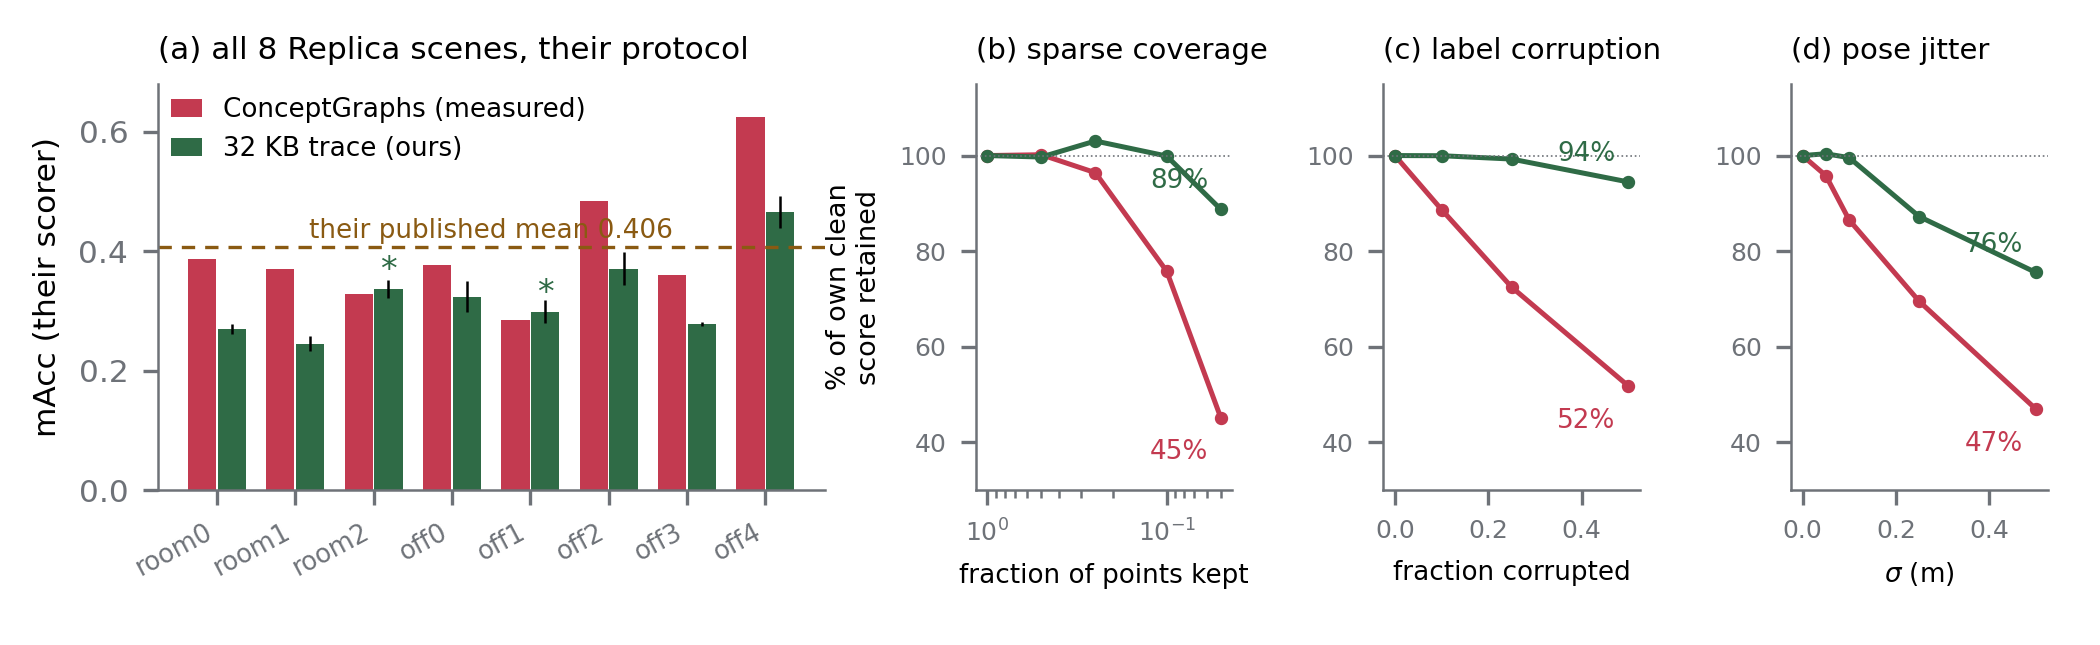
\includegraphics[width=\textwidth]{figures/replica_headtohead.png}
% provenance: tools/make_replica_headtohead_figure.py from
% outputs/batch1/table2_full.json + outputs/degradation_sweep.json
\caption{The head-to-head and the crossover. \textbf{(a)} mAcc per scene
under ConceptGraphs' own scorer and exclusion protocol: their released
system re-measured (red) against one fixed 32\,KB trace per scene
(green, error bars = sd over 5 seed draws); dashed line, their published
8-scene mean; stars, scenes the trace wins outright.
\textbf{(b--d)} Fraction of each system's \emph{own} clean score
retained as the shared input degrades (\texttt{room0} shown; the pattern
is unanimous over 3 scenes $\times$ 3 modes, and every sweep ends with
the trace ahead in absolute score). The bounded memory starts 20\%
behind and finishes ahead everywhere: degradation, not peak accuracy, is
where the representations separate.}
\label{fig:headtohead}
\end{figure*}

\subsection{Two properties that follow from the algebra}
\label{sec:merge-results}

\textbf{Merge.} Four session memories built independently from the four
\texttt{chess} training traverses and summed agree with the jointly built
trace to max $|\Delta| = 1.6\times10^{-15}$ and answer all 2{,}000 test
queries identically --- exactness in a checkable sense, with zero
association decisions.
% provenance: tracker (ax), merge check in cross_recall.py --merge-check
A measured comparison against instance-association merging over identical
observations, and against VSA-OGM's occupancy fusion on its own
benchmark, is the subject of a companion paper.

\textbf{Drift bounding.} Both steps of a Kalman-style filter are native
to the algebra: predict is one bind ($O(D)$, no grid), update is one
bundle. Under a 20$\times$ odometry-degradation sweep on the classroom
sequence, dead reckoning diverges to 17.6\,m while the fused estimate
saturates at 0.62\,m, approximately the memory's own recall accuracy.
% provenance: tracker (ag),(ah); vsa_kalman_seeds.json
The honest claim is not that the memory out-localises odometry --- raw
recall (median 0.62\,m) does not reliably beat low-noise dead reckoning
(0.87$\pm$0.50\,m over 10 noise seeds; dead reckoning wins 5 of 10) ---
but that a fixed-size associative memory caps unbounded drift at $O(D)$
per frame.

% =========================================================================
\section{Limitations}
\label{sec:limitations}

\textbf{Instance identity.} Binding class$\bnd$position recalls
\emph{class} fields: on multi-instance classes the argmax lands on the
wrong instance 72\% of the time (1{,}309 held-out instance queries, 5
scenes). An appearance-keyed variant raises instance accuracy to 43\% and
a hybrid cuts outright errors to 3\%, but part of the residual is
Replica's genuinely identical instance models. Systems with explicit
relational structure \cite{farm2026} hold this frontier.

\textbf{Vocabulary and metric coverage.} The object memory sees what its
frontend sees (9--31\% of Replica GT instances under COCO-80) and cannot
label structure classes; the pre-registered expectation under the dense
all-classes metric was accordingly low and was confirmed
($\approx$0.076 on \texttt{room0}). The head-to-head of
Sec.~\ref{sec:grounding} removes this confound by feeding both memories
the same frontend --- and its forensics show 62\% of our remaining
losses originate in that shared stream's label placement, a ceiling no
memory backend can raise.

\textbf{The shared frame.} Merge exactness assumes a shared coordinate
convention; frame recovery inside the algebra is built but its robustness
under partial overlap is unmeasured, so no claim is made.

\textbf{Scale and scope.} Room-scale scenes, $\sim$10$^4$ observations per
trace, one self-collected platform. Whitening's harm and heading's value
are scene- and trajectory-dependent and stated as scoped claims. Absolute
recall is honest-modest everywhere: the memory tracks its frontend's
ceiling and does not exceed it.

% =========================================================================
\section{Conclusion}
\label{sec:conclusion}

We characterised a spatial-semantic map whose entire state is one
fixed-size vector, and located its contribution in the law that governs
it rather than in its size. Insertion is a multiply-add, a family of
object/place/time queries is one unbind each, and merging is elementwise
addition. On a public relocalisation benchmark the trace recalls within
0.07\,m of exact nearest neighbour at $\sim$1000$\times$ fewer bytes, in
a size regime standard compression cannot enter; on eight Replica scenes
its grounding misses are entirely attributable to perception; and
against a reproduced ConceptGraphs baseline under that system's own
evaluation it holds 0.80$\times$ the accuracy of an unbounded map on
clean input and overtakes it outright in every degraded-input condition
tested. Its
interference is governed by a capacity law precise enough to predict a
held-out condition to 1.4\% and to have called a deployed failure and its
fix in advance --- and that law is also the deployment discipline that
makes the algebra work on real learned features.

The trade is stated as plainly as the wins: the representation is
bounded, associative and approximate, where scene graphs are exact,
mutable and relational, and recent work shows explicit structure can be
small too. It does not solve the shared-frame problem its merge operator
assumes; it does not individuate identical instances; its recall ceiling
is its perception's. What it offers is a map whose costs are known in
advance --- bytes fixed before deployment, update cost independent of map
age, merge cost independent of map content --- and, unlike other bounded
memories, failure modes predicted by an equation rather than discovered
in the field.

% =========================================================================
\section*{Acknowledgments}
This work was begun at the 2026 Telluride Neuromorphic AI Workshop, and
the authors thank its organisers and participants for the environment in
which the collaboration was formed. The material in this paper is based
upon work supported by the National Science Foundation under BCS 1824198,
OISE 2020624, and ECCS-2332166, and by ONR grant N00014-24-1-2025. Any
opinions, findings, and conclusions or recommendations expressed in this
publication are those of the authors and do not necessarily reflect the
views of the National Science Foundation.
\todo{institutional funding for each author}

\bibliographystyle{IEEEtran}
\bibliography{refs}

\end{document}
